\documentclass[xcolor=dvipsnames,aspectratio=169]{beamer}
\usepackage{xcolor}
\usepackage{hyperref}

\usepackage[utf8]{inputenc}
\usepackage{multicol}
\usepackage{utopia} %font utopia imported
% \usetheme{Madrid} %Madrid %Berkeley
\usetheme[width=1.5cm]{Madrid} 
\definecolor{RBlue}{RGB}{44, 108, 188} 
\usecolortheme[named=RBlue]{structure}
\usepackage{listings}


%------------------------------------------------------------
%This block of code defines the information to appear in the
%Title page
\title[]{A Gentle Introduction to Modern Optimization Tools in R}

\subtitle{rcbc \& minizinc 
}

\author[]{Shuai Wang \and Eugene Pyatigorsky}

\institute[] % (optional)
{84.51 Operations Research}

\date[] % (optional)
{CinDay R User Meetup, May 22 2019}

\logo{
\includegraphics[height=1.5cm]{CinDayR_logo.png}}

%End of title page configuration block
%------------------------------------------------------------



%------------------------------------------------------------
%The next block of commands puts the table of contents at the 
%beginning of each section and highlights the current section:

\AtBeginSection[]
{
  \begin{frame}
    \frametitle{Table of Contents}
    \tableofcontents[currentsection]
  \end{frame}
}
%------------------------------------------------------------


\begin{document}

%The next statement creates the title page.
\frame{\titlepage}


%---------------------------------------------------------
%This block of code is for the table of contents after
%the title page
\begin{frame}
\frametitle{Table of Contents}
\tableofcontents
\end{frame}
%---------------------------------------------------------


\section{Mathematical Optimization}

%---------------------------------------------------------
\begin{frame}
\frametitle{What's mathematical optimization anyway?}

\begin{itemize}
    \item “Optimization” comes from the same root as “optimal”, which means best. When you
optimize something, you are “making it best”.
 
 
\item But “best” can vary. If you’re a football player, you might want to maximize your
running yards, and also minimize your fumbles. Both maximizing and minimizing are types
of optimization problems.
\end{itemize}



\end{frame}

%---------------------------------------------------------


%---------------------------------------------------------
%Example of the \pause command
\begin{frame}
\frametitle{Mathematical Optimization in the “Real World”}
Mathematical Optimization is a branch of applied mathematics which is useful in many different fields. Here are a few examples:
 \begin{multicols}{2}
    \begin{itemize}
        \item Manufacturing
        \item Production
        \item Inventory control
        \item Transportation
        \item Scheduling
        \item Networks
        \item Finance
        \item Economics
        \item Control engineering
        \item Marketing
        \item Policy Modeling
        \item Mechanics
    \end{itemize}
    \end{multicols}

\end{frame}


\begin{frame}{Optimization Model Components}
Your basic optimization problem consists of: 
\begin{enumerate}
    \item The objective function, {\color{red} f(x)}, which is the output you’re trying to maximize or minimize. e.g. maximize the gross profit margin; minimize travel distance of a pizza delivery car. 
    
    \item  Variables,  {\color{red}$x_1, x_2, x_3$} and so on, which are the inputs – things you can control. 
    
    \item Constraints, which are equations that place limits on how big or small some variables can get. e.g. The pizza delivery should be on time.
    
    
\end{enumerate}


\end{frame}


\begin{frame}{Optimization Example}
    A football coach is planning practices for his running backs.
\begin{itemize}
    \item His main goal is to maximize running yards – this will become his
    {\color{red} objective function}.
    
    \item He can make his athletes spend practice time in the weight room; running 
    sprints; or practicing ball protection. The amount of time spent on each is a 
    {\color{red} variable}.
    
    \item  However, there are limits to the total amount of time he has. Also, if he
    completely sacrifices ball protection he may see running yards go up, but also 
    fumbles, so he may place an upper limit on the amount of fumbles he considers 
    acceptable. These are {\color{red} constraints}.
\end{itemize}

Note that the variables influence the objective function and the constraints place limits on the domain of the variables.
\end{frame}


%---------------------------------------------------------
\section{Using R to model optimization problem}

\begin{frame}{Knapsack problem}
\begin{itemize}
    \item You only bring one knapsack with a capacity 
    limit to rob a bank. 
    \item Different gold has various amount of 
    value and weight.
    \item Try to get as much value as possible.
    \item So, which ones to choose with the capacity limit of the 
    knapsack. 
\end{itemize}

\begin{figure}
\centering

\vspace*{-0.5cm}
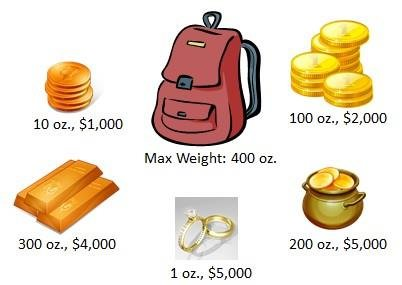
\includegraphics[scale=0.6]{knapsack-problem.png}

\end{figure}
\end{frame}


\begin{frame}{Knapsack problem math modeling}
KP has the
following Integer Linear Programming (ILP) formulation:

\begin{gather}
\text{maximize \ \ \ }\sum_{j\in N}p_{j}x_{j}\text{ \ \ \ \ \ \ \ }
\label{eq:ILP1} \\
\text{subject to \ \ }\sum_{j\in N}w_{j}x_{j}\leq c  \label{eq:ILP2} \\
\text{ \ \ \ \ \ \ \ \ \ \ \ \ \ \ \ \ \ \ \ \ \ \ \ \ \ }x_{j}\in \{0,1\},%
\text{ \ \ }j\in N,  \label{eq:ILP3}
\end{gather}%
where each binary variable $x_{j}$, $j\in N$, is equal to 1 if and only if
item $j$ is selected.
$p_{j}$: price/value of each item; $w_{j}$: weight of each 
item. 

We cannot take all items because the total
weight of the chosen items cannot exceed the knapsack 
capacity $c$.
    
\end{frame}

\begin{frame}{Common solvers for linear and integer optimization problems}
\begin{multicols}{2}

\textbf{Commercial:}
\begin{itemize}
    \item IBM CPLEX 
     \item Gurobi
     \item FICO EXPRESS
     \item MOSEK
\end{itemize}
    
\textbf{Open-Source:}

\begin{itemize}
    \item SCIP (commercial use restriction)
    \item GLPK 
    \item COIN-OR /CBC
    \item COIN-OR/SYMPHONY
\end{itemize}
\columnbreak
        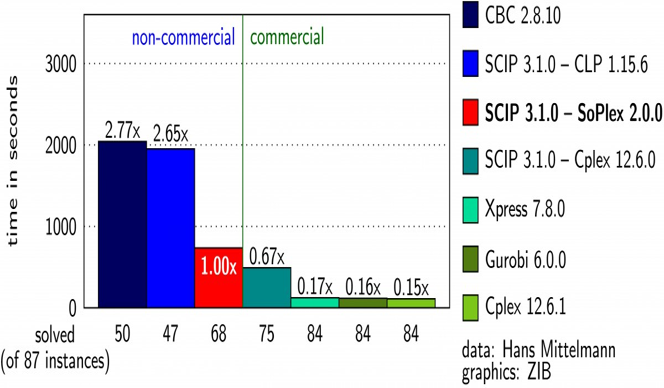
\includegraphics[width=80mm, height = 70mm ]{benchmark.png}

\end{multicols}
\end{frame}


\begin{frame}{Solver Benchmark}
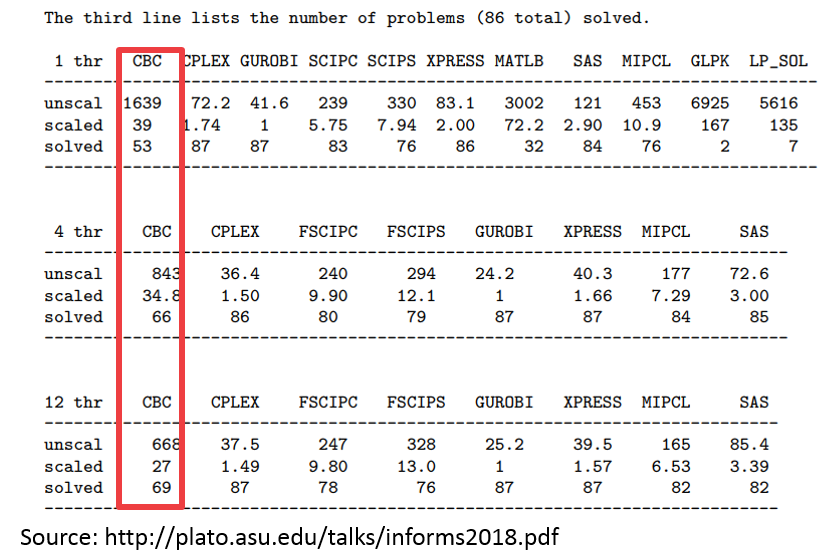
\includegraphics[width=140mm, height = 60mm]{benchmark2.PNG}
    
\end{frame}


\begin{frame}{Using library(rcbc)}


https://github.com/dirkschumacher/rcbc

\begin{figure}[t]
  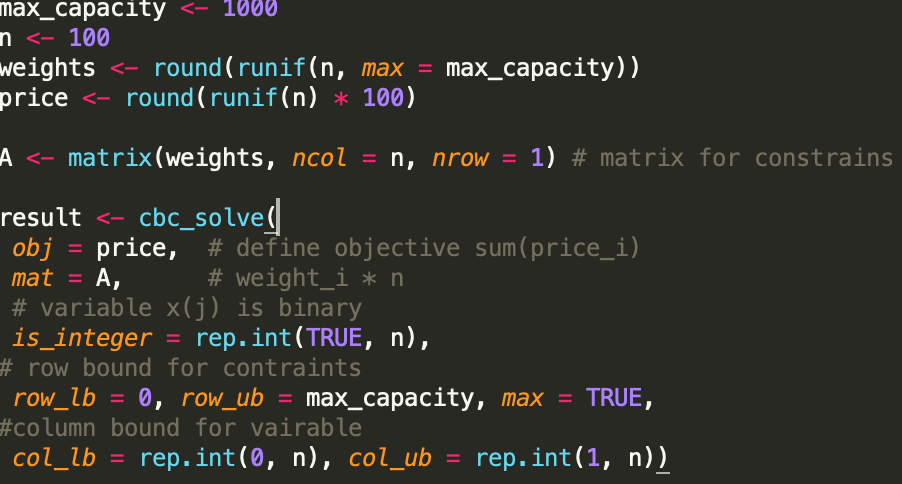
\includegraphics[height =6.5cm]{knapsack.png}

\centering
\end{figure}
\end{frame}



\begin{frame}{Minizinc: The Right Tool for the Right Job.}
Minizinc is a free and open-source constraint modeling language.

You can use Minizinc to model constraint 
satisfaction and optimization problems in a 
high-level, solver-independent way.

    \begin{figure}
    \centering
        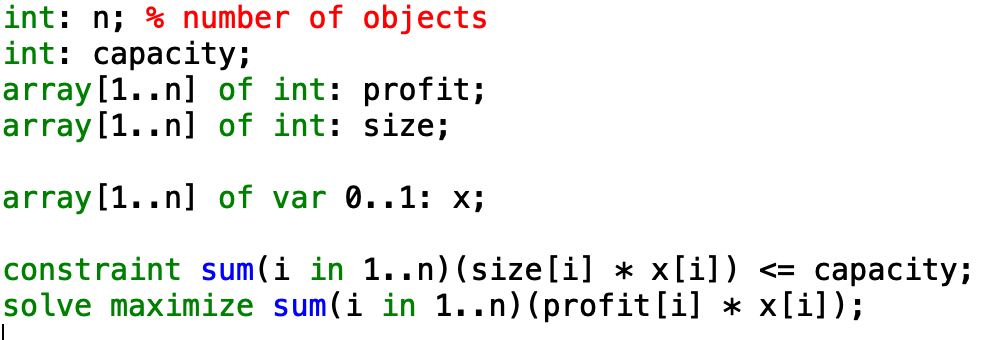
\includegraphics[height =4.4cm]{Minizinc_knapsack.png}
    \end{figure}
\end{frame}


\begin{frame}{Knapsack problem application}
    
In any real-world problems where you have resources with certain values
and you want to waste as little as possible.
    \begin{itemize}
        \item Shipping containers, to be packed as efficiently as possible.
        \item To cut large  pieces of materials into smaller packages (paper, metal, wood-logs).
        \item To optimize portfolios (which shares and how 
        many should you buy).

    \end{itemize}

\end{frame}

\begin{frame}{A Typical Resource Planning Problem}
        \begin{itemize}
            \item  How much of each kind of product to make to maximize profit where manufacturing a product consumes varying amounts of some fixed resources
            \item Minizinc uses a data file with non-standard format
            \begin{multicols}{2}
            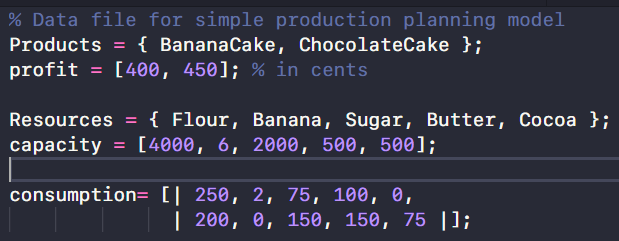
\includegraphics[width = 70mm ]{mz_production_data.png}
            \columnbreak
            
            
\includegraphics[width = 40mm]{cake.jpg}
            \end{multicols}
        \end{itemize}

\end{frame}

\begin{frame}{Easy to Express in Minizinc}
    \begin{figure}[t]
     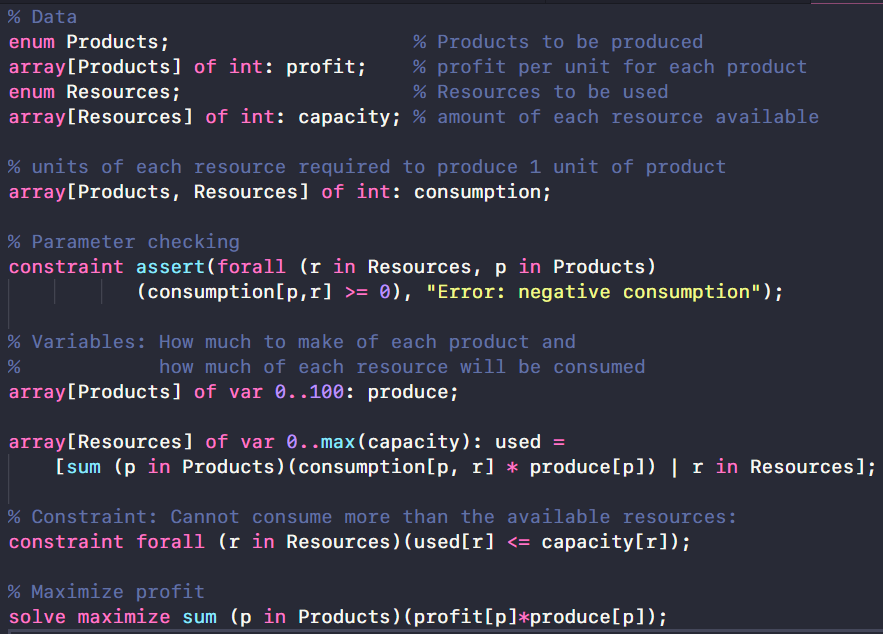
\includegraphics[height = 70mm, pos = center]{mz_production_model.png}
    \centering
    \end{figure}
\end{frame}

\begin{frame}{Minizinc with R: Data Templates}
   \begin{itemize}
    \item We treat the data file (dzn) as a template to be filled in by R, using handmade casting functions
    \item `glue` does the string interpolation
    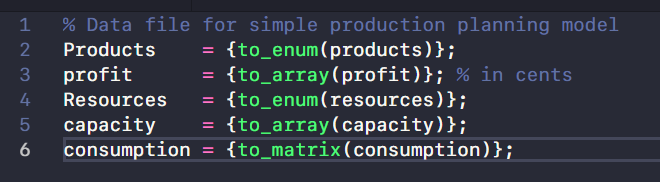
\includegraphics[scale = 0.65]{mz_production_data_2.png} 
   \end{itemize}
    
\end{frame}

\begin{frame}{Minizinc with R: Calling the Executable}
   \begin{itemize}
    \item A thin wrapper on top of the minizinc command line executable passes in the model and data files and receives a json-formatted result. 
    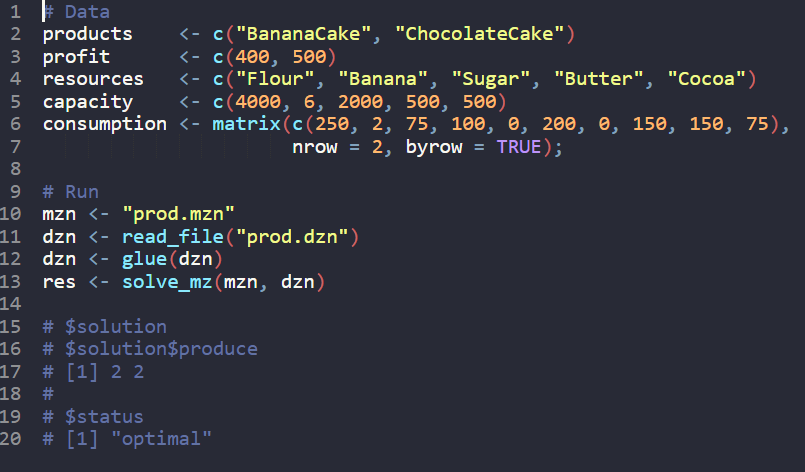
\includegraphics[scale = 0.60]{mz_production_result.png} 
   \end{itemize}
    
\end{frame}

\begin{frame}
 %\begin{multicols}{2}
    Thank you!
%\columnbreak
\begin{figure}
    \centering
   
\includegraphics[scale = 0.5]{thank_you.JPG}
\end{figure}
% \end{multicols}
\end{frame} 

\end{document}